\documentclass[review]{elsarticle}
\usepackage[colorlinks]{hyperref}
\usepackage[colorinlistoftodos]{todonotes}
\usepackage{verbatim}
\usepackage[utf8]{inputenc}
\usepackage[T1]{fontenc}
\usepackage{adjustbox}
\usepackage{multirow}
\usepackage{longtable}
\usepackage{booktabs}
\usepackage{lineno,hyperref}
\modulolinenumbers[5]

\journal{Science \& Technology of Archaeological Research}

%%%%%%%%%%%%%%%%%%%%%%%
%% Elsevier bibliography styles
%%%%%%%%%%%%%%%%%%%%%%%
%% APA style
\bibliographystyle{model5-names}\biboptions{authoryear}
%%%%%%%%%%%%%%%%%%%%%%%

\begin{document}

\begin{frontmatter}

\title{Shape as a function of time + raw material + burial context: A preliminary analysis of Perdiz arrow point shape from the southern Caddo area}

%% Group authors per affiliation:
\author{Robert Z. Selden, Jr.\textsuperscript{a,b,c}*, John E. Dockall\textsuperscript{d,e}, C. Britt Bousman\textsuperscript{f,g}, and Timothy K. Perttula\textsuperscript{h}}
\address[1]{Heritage Research Center, Stephen F. Austin State University, US}
\address[2]{Cultural Heritage Department, Jean Monnet University, FR}
\address[3]{ORCID ID \href{http://orcid.org/0000-0002-1789-8449}{0000-0002-1789-8449}}
\address[4]{Cox|McClain Environmental Consulting, Inc., US}
\address[5]{ORCID ID \href{http://orcid.org/0000-0002-0940-7144}{0000-0002-0940-7144}}
\address[6]{Department of Anthropology, Texas State University, US}
\address[7]{ORCID ID \href{http://orcid.org/0000-0002-1645-8302}{0000-0002-1645-8302}}
\address[8]{Archeological \& Environmental Consultants, LLC, US}
\cortext[cor1]{Corresponding author, Robert Z. Selden, Jr. (zselden@sfasu.edu)}

\begin{abstract}
Temporal assignments carry substantive weight in archaeological practice, and it is regularly assumed that artifacts from different temporal units may have differed in ways that convey changes in preference or behaviour. Similarly, archaeologists regularly assume that raw material differences articulate with stone tool morphology, and the role of differential raw material quality and preference associated with Caddo lithic technology remains largely unexplored. Whether a particular artefact is found within or outside of burial contexts is a sensitive and regularly discussed topic in the archaeological literature, providing valuable insights related to prehistoric burial practices, as well as generational shifts in aesthetics, design, and raw material preference. These assumptions were tested using the tools of geometric morphometrics, yielding results that support the hypothesis that Perdiz arrow point shape is protean, and that significant differences existed in shape by time, raw material choice, and burial context.
\end{abstract}

\begin{keyword}
Caddo, NAGPRA, computational archaeology, museum studies, digital humanities, STEM
\end{keyword}

\end{frontmatter}

\linenumbers

\section*{}

\begin{quote}
The assumption is that the ability to execute formal technological designs is severely limited by the quality of the raw material. Toolkits based on high quality raw materials are thought to be easier to design because fracture is easier to control \citep{RN4315,RN8924}. In contrast, toolkits based on poor quality raw material are more difficult to design because fracture is unpredictable and results in severe, irreparable errors during reduction. Even where low raw material abundance would encourage formal technological design, raw material quality is thought to be the overriding factor constraining lithic technological organization \citep[257]{RN5907}.
\end{quote}

East Texas geologic formations are poor in lithic raw materials \citep[Figure 2.1]{RN439}, or at least knappable lithic materials. Consequently, lithic materials suitable for the manufacture of Perdiz arrow points would have been a carefully conserved resource for the sedentary aboriginal Caddo populations that lived in East Texas. In the general East Texas area, only the Pisgah Ridge chert in the Trinity River basin, Manning fused glass in the Manning Formation (part of the Jackson group of Eocene age), and various cherts and quartzites in the Catahoula Formation (exposed in the Neches River basin) are in “geological formations that contain in situ rocks suitable for the manufacture of stone tools” \citep[49]{RN439}. There are also upland stream gravels that are relatively widespread in parts of East Texas \citep[56-57]{RN439}. High quality and knappable cobbles of chert, novaculite, and quartzite are present in the Red River gravels in northeastern Texas (as well as in the Bowie gravels in the Red-Sulphur River interfluve, per \citet{RN846}), and these derive from chert-bearing formations in the Ouachita Mountains of southeastern Oklahoma \citep[Figure 1.20]{RN439}.

According to a study of lithic raw material sources in the Neches-Angelina river basin \citet[69]{RN1253}, there are redeposited gravels on stream terraces that contain small cobbles and pebbles of petrified wood, fine-grained quartzite, and various cherts. The local cherts tend to be red, gray, tan, and brown in color \cite[66]{RN1253}. Non-local cherts found on sites in the Neches and Angelina river basins are apparently from Central Texas Edwards Plateau sources, and these are lustrous gray, blue-gray, and dark brown in colour.

Local lithic raw materials include coarse- and fine-grained quartzite, petrified or silicifed wood, ferruginous sandstone, jasper, and several varieties of earth-toned cherts: yellowish-brown, gray, red, light brown, brown, greenish-brown, and a reddish-brown color. Non-local raw materials are white and red novaculite, black chert, dark gray chert, white chert, bluish-gray chert, a yellowish-red chert, and quartz. A distinctive coarse-grained quartzite (or metaquartzite) may occur in this general area, though it probably is restricted to localised sources. The material is described by \citet[67]{RN1253} as being of sugary coarse-grained texture and light gray to yellowish-brown in colour, and may originate in the Glover Sandstone (part of the basal Sparta Sand Formation) in northeastern Houston County \cite[69]{RN1253}. A quarry (41VN39) of grayish-white quartzite is known in the Sabine River basin in Van Zandt County, and has been noted to turn pink when heat-treated \cite{RN1898}).

The most likely contributing source(s) of non-local cherts used for the manufacture of Perdiz arrow points in northeast and east Texas are those from various Edwards Formation localities in central Texas \citep{RN439,RN2145}. These resources occur in a region that encompasses the Edwards Plateau and the southern Llano Estacado and occur in both massive ledge and cobble varieties. These materials also occur as significant gravel sources along the Colorado and Brazos River Valleys but may also occur as reworked and lagged members of Uvalde Gravel deposits.

\subsection*{Shape, raw material, and human behaviour}

Perdiz arrow points (\citealp[283 and Plate 142]{RN7795}; \citealp[504 and Plate 131]{RN5769}) occur across most of Texas from the Rio Grande eastward to the Neches River basin, and from the Red River (Texas and Oklahoma) south to the eastern and central parts of the Gulf Coast, and have been noted to include more variation in size and proportions than most arrow point types in Texas. In outline, Perdiz arrow points have a “[t]riangular blade with edges usually quite straight but sometimes slightly convex or concave. Shoulders sometimes at right angles to stem but usually well barbed. Stem contracted, often quite sharp at base, but may be somewhat rounded. Occasionally, specimen may be worked on one face only or mainly on one face…[w]orkmanship generally good, sometimes exceedingly fine with minutely serrated blade edges” \cite[504]{RN5769}. 

Perdiz arrow points fall within what \citet[738-741]{RN5873} referred to as a maintainable tool; however, unlike dart points, the morphological attributes of arrow points—generally small and thin—somewhat limit discussions of optimisation related to planned breakage caused by impact \citep{RN6170,RN7045}, providing for differing expressions of maintainability \citep{RN5789}. The anticipated exploitation of raw material resources, coupled with the perceived technological advantages of using heat treatment \citep{RN6171} , may have resulted in longer and larger flakes (and more of them), provided the temperature of the stone reached the requisite temperature \citep{RN5900}. Thermal properties of locally-available raw materials are ill-understood in the southern Caddo area, and it remains unclear whether Caddo knappers enlisted expedient \citep{RN8970,RN6201}, slow and steady \citep{RN8971}, or hybrid approach to heat treatment.

Inferences regarding human behaviour drawn from stone tool raw material source use patterns are predicated on accurate knowledge of the location of sources actually used \citep[365]{RN5787}. Reduction models rooted in knapping experiments make an assumption that the reduction process is known \citep{RN6855}; however, experiments have illustrated that numerous manufacturing strategies could be employed to generate the same products \citep{RN8968,RN8969}. 

\section*{Perdiz arrow point sample}

The Perdiz sample used in this analysis comes from Camp, Harrison, Nacogdoches, San Augustine, Smith, and Shelby counties, and consists of whole/intact Perdiz arrow points from 10 sites across the southern Caddo area, which were manufactured using chert, jasper, quartzite, and silicified wood (Figures map and int1:a). Raw material distributions differ among the sites where chert occurs across the greatest geography (Figure int1:a). Use of quartzite and jasper were limited to Camp County, where jasper Perdiz arrow points were recovered only at the Tuck Carpenter site (41CP5) (Figure int1:a). Silicified wood was employed for Perdiz manufacture in Nacogdoches and Shelby Counties; however, Washington Square Mound (41NA49) is the only burial context where silicified wood Perdiz points have been recovered (Figure int1:a). While the full range of these raw materials were used in Caddo burials, only chert and silicified wood points were found to occur outside of burial contexts (Figure int1:b). Raw materials also differ through the Middle, Late, and Historic Caddo periods, where chert and silicified wood are present throughout all three periods; while jasper and quartzite occur only in Middle Caddo mortuary contexts (Figure int1:c). Radiocarbon and relative dates are discussed in more detail below; however, the median of that temporal range was used to assign the Perdiz points to the appropriate temporal period (Middle Caddo, A.D. 1200-1450; Late Caddo, A.D. 1450-1680; and Historic Caddo, A.D. 1680+) (Figure int1:d).

\begin{figure}[!]\centering
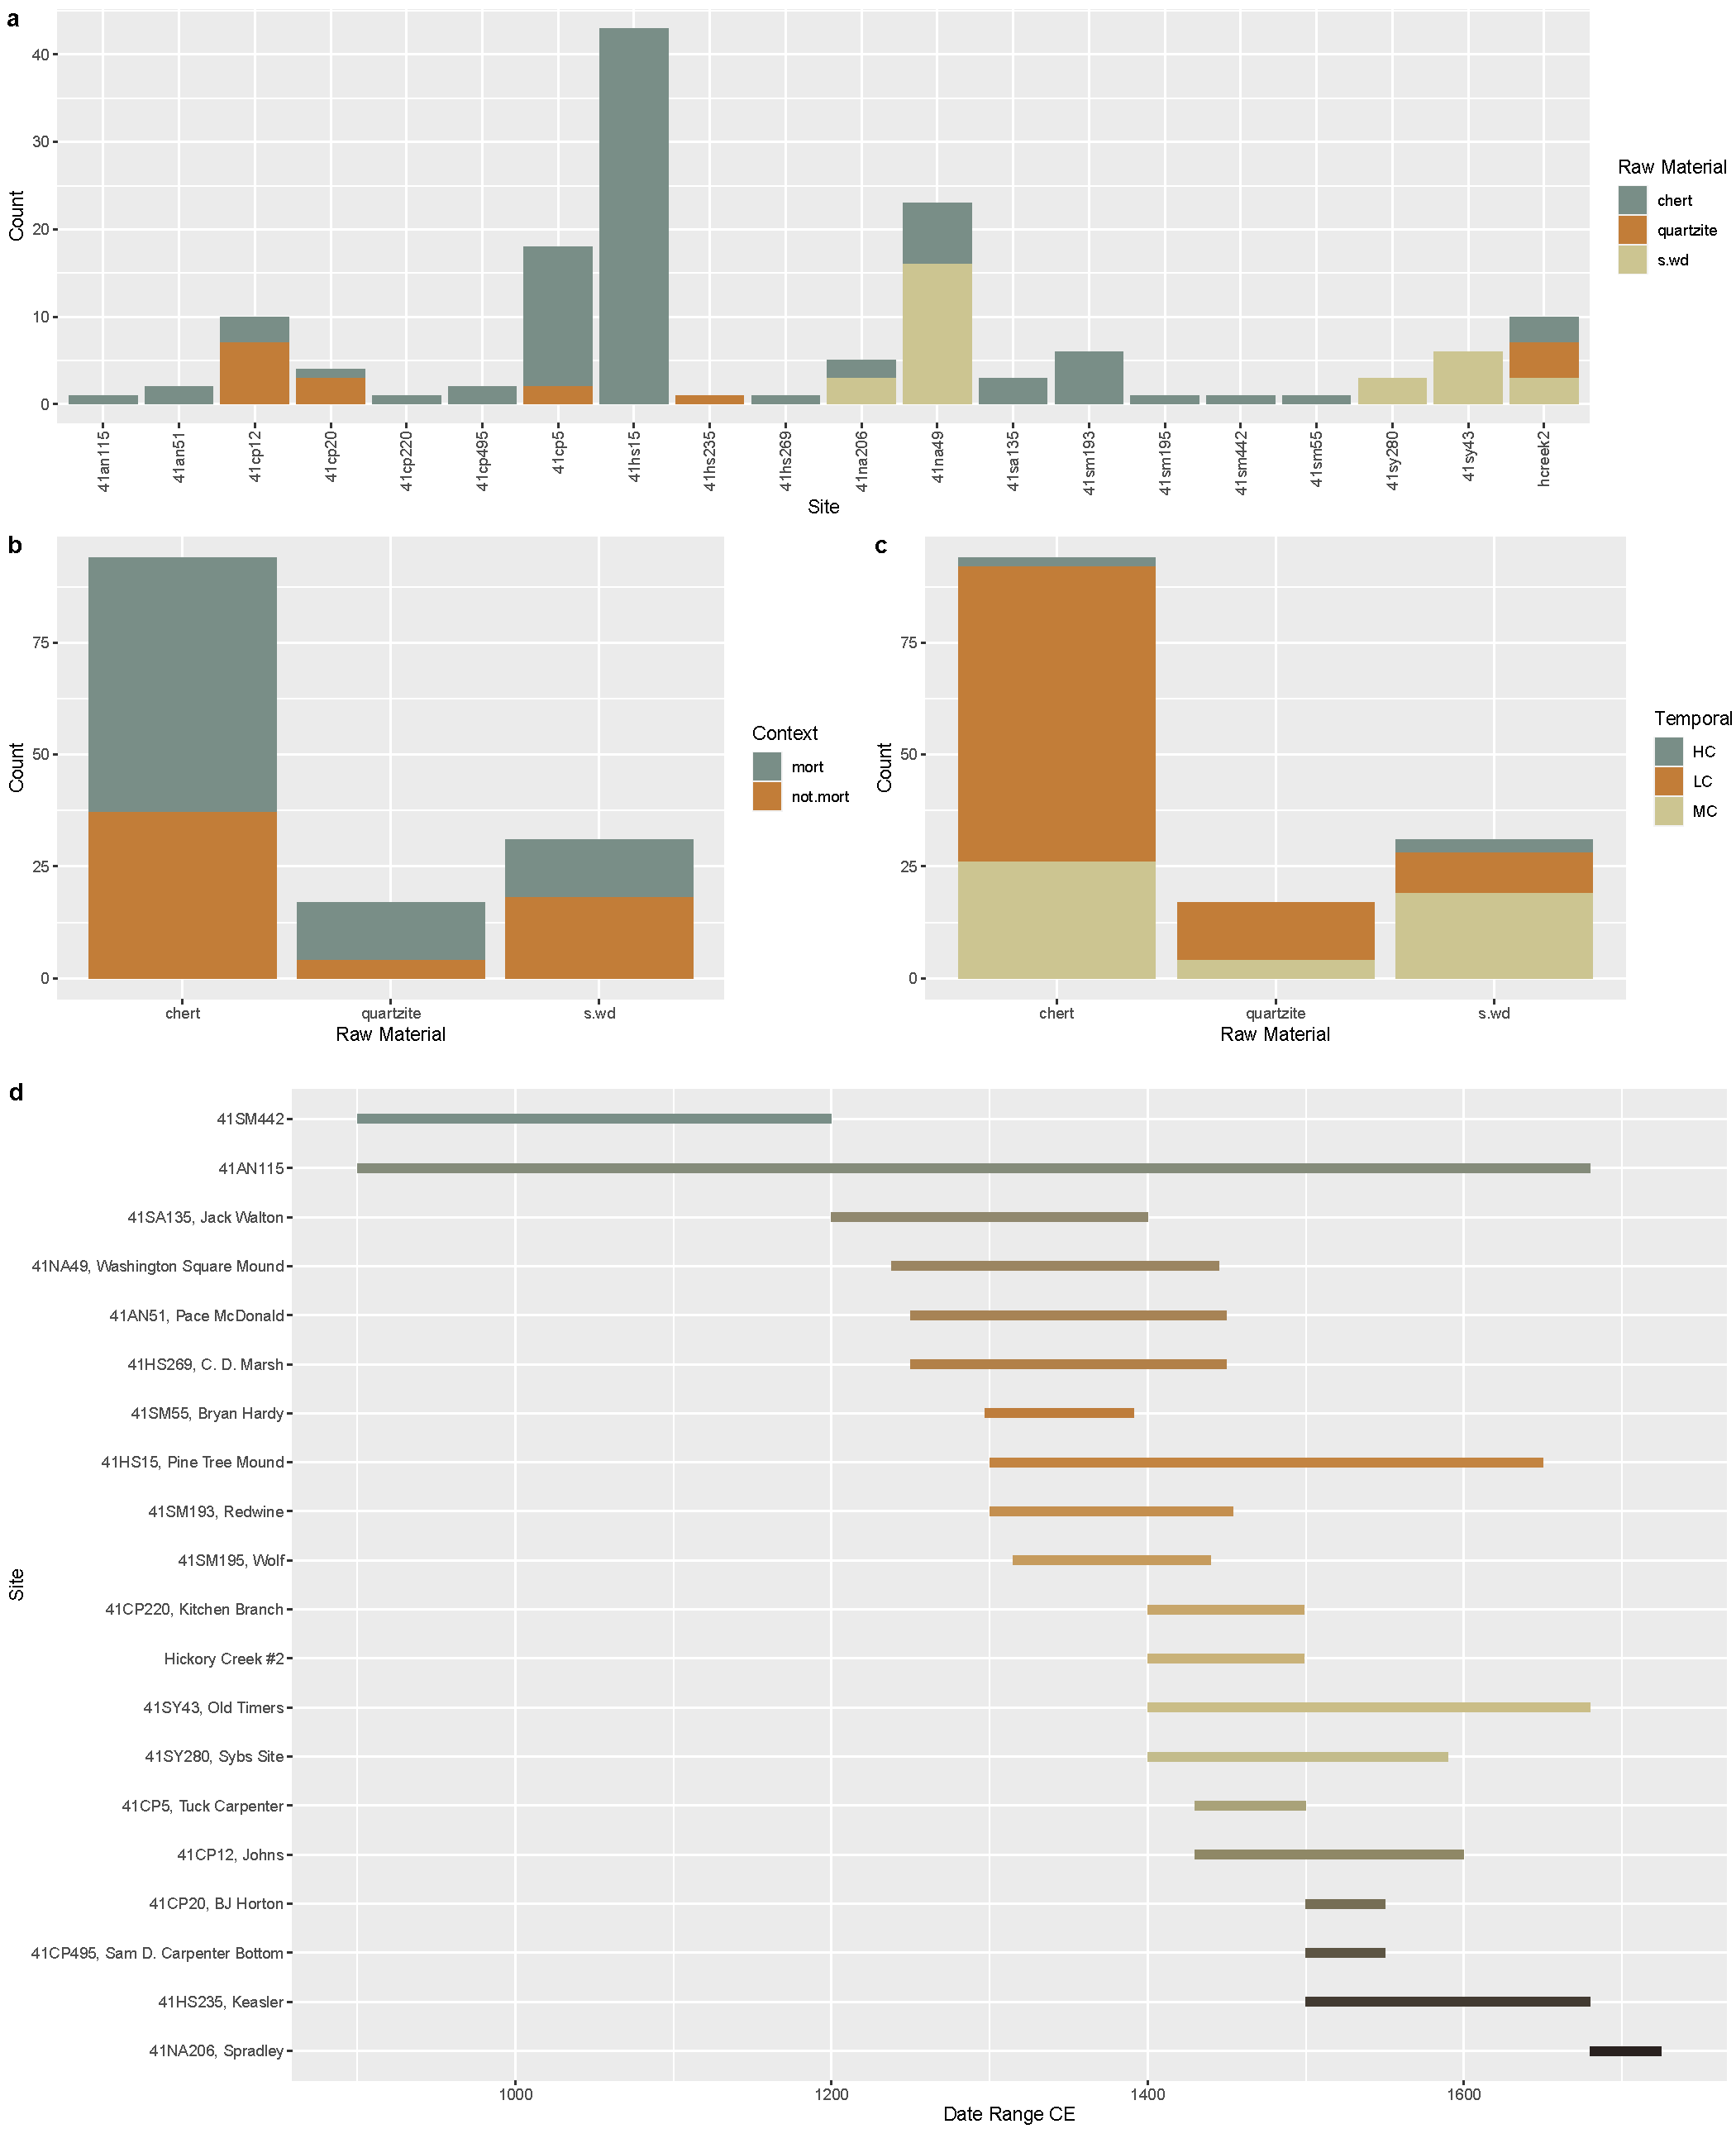
\includegraphics[width=\linewidth]{fig.mat.temp.pdf}
\caption{Raw materials a, by site; b, by mortuary context; c, by temporal period (Middle, Late, or Historic Caddo), and d, temporal span of contexts in the Perdiz sample}
\label{fig:raw.mat}
\end{figure}

\subsection*{41CP5, Tuck Carpenter}

The Tuck Carpenter site is a well-studied Late Caddo period Titus phase cemetery on Dry Creek in the Big Cypress Creek basin, and was occupied by the Caddo from the 15th to the 17th century A.D. Burials with Perdiz points are the earliest in the cemetery, and likely date from A.D. 1430-1500 (Perttula, et al. 2017:197). A single radiocarbon date was obtained from Burial 10: 360 + 60 B.P. The calibrated age range at 2 sigma is A.D. 1442-1646, with a median probability of A.D. 1546 (using INTCal 20 and Calib 8.20).

Fifty seven Perdiz points have been recovered from burial features at the Tuck Carpenter site (Perttula 2009; Turner 1978, 1992). A second collection from the site includes an additional 18 Perdiz points from 13 of the burial features  made from Ogallala quartzite and local chert gravel sources; including one that was made from a non-local novaculite (Perttula, et al. 2017:Table 2).

\subsection*{41CP12, Johns}

The Johns site is a Titus phase cemetery in the Prairie Creek valley in the Big Cypress Creek basin. No radiocarbon dates have been obtained from the site, but the decorative motifs associated with the ceramic vessels recovered from burials suggest that the cemetery was used from A.D. 1430-1600 (Perttula, Walters, et al. 2010b). Forty-eight Perdiz points were recovered from 16 burial features. They were made from local chert, quartzite, and petrified gravel sources (87 percent), non-local sources (10.8 percent, mainly from Red River gravels), and chalcedony (2.2 percent).

\subsection*{41CP20, B. J. Horton Site}

This ancestral Caddo cemetery in the Big Cypress Creek basin includes at least 19 burials, from which two Perdiz points were recovered (Perttula, Walters, et al. 2010a:9). Use of the cemetery by the Caddo occurred primarily between A.D. 1500-1550 (Perttula and Miller 2014:494).

\subsection*{41HS15, Pine Tree Mound Site}

The Pine Tree Mound site is a large Titus phase mound center with associated habitation deposits, family cemeteries, and a large community cemetery (Fields and Gadus 2012). Perdiz arrow points (n = 68) represent 53 percent of the arrow points that could be typed from the site, most (n = 50) from burial contexts and the remainder from habitation deposits. Perdiz points from burial contexts tend to have been made from non-local lithic raw materials, typically chert (42 percent), while none of the non-mortuary Perdiz points are made on non-local raw material (Fields and Gadus 2012:566) (Fields and Gadus 2012:566).

There are 92 radiocarbon dates available from the Pine Tree Mound site (Fields and Gadus 2012:Table 4.13; Selden Jr. and Perttula 2013:Table 2). Most of the calibrated dates fall between A.D. 1451-1495 and A.D. 1397-1429 (Selden Jr. and Perttula 2013:Table 3), but calibrated age ranges suggest that the settlement “was established in the A.D. 1300s and persisted until at least the mid 1600s” (Fields and Gadus 2012:299).

\subsection*{41NA49, Washington Square Mound}

The Washington Square Mound site is located in the Angelina River basin and is a mound center with associated habitation deposits and a cemetery. Excavations in one mound uncovered two shaft tombs with abundant grave goods, but no Perdiz offerings (Corbin and Hart 1998; Perttula, Walters, Nelson, et al. 2010). However, 14 Perdiz points were recovered from a burial feature in the Oak Grove Cemetery portion of the Washington Square Mound site (Perttula, Walters, Nelson, et al. 2010:Figure 77). Another seven Perdiz points came from habitation areas near the main burial mound  (Perttula 2009:Table 14). Of those, 71 percent are on gray chert of likely central Texas origin, and the remainder were made from local quartzite.

Twelve radiocarbon dates have been obtained from the Washington Square Mound site (Corbin and Hart 1998:Table 4; Selden Jr. and Perttula 2013), indicating use of the site in both Early (A.D. 900-1200) and Middle Caddo periods. The best dates that can be associated with Perdiz points at the site range from cal. A.D. 1238-1445.

\subsection*{41NA206, Spradley}

The Spradley site includes late 17th to early 18th century archaeological deposits with European trade goods from habitation deposits in the Bayou La Nana valley in the Angelina River basin (Perttula and Marceaux 2018). Those habitation deposits, which have no associated radiocarbon dates, contain numerous Perdiz points (n = 31). Approximately 94 percent were manufactured from local silicified wood, quartzite, and gravel cherts, and the remainder are from non-local brownish-gray to translucent gray chert, likely from central Texas raw material sources (Perttula and Marceaux 2018:Table 7).

\subsection*{41SA135, Jack Walton Site}

This site is located on Attoyac Bayou (Middlebrook 2010), and is an ancestral Caddo site with habitation deposits of likely Middle Caddo period age (A.D. 1200-1400). There are no radiocarbon dates from the site. Excavations at the site recovered seven Perdiz points.

\subsection*{41SM193, Redwine}

The Redwine site (41SM193) site is a Middle Caddo period component located 22 km from the river on a north-flowing tributary (Auburn Creek) of the Sabine River (Walters and Haskins 1998), which includes habitation deposits and a small cemetery. The site has one calibrated date of A.D. 1300-1454, at 2 sigma, with a median calibrated probability of A.D. 1356. The 11 Perdiz points from habitation deposits were manufactured on black, brown, and grayish-tan chert as well as Ogallala quartzite (Walters and Haskins 1998:14). An additional 13 Perdiz arrow points were among the grave goods recovered from two burial features (Walters and Haskins 1998:35).

\subsection*{41SY43, Old Timers Site}

The Old Timers site is located in the Sabine River basin, and includes post-A.D. 1400 Late Caddo habitation deposits concentrated in the northern area of the site. Excavations recovered eight Perdiz points, all with serrated blades and made from cherts, 75 percent local gravel cherts, and an additional 25 percent of gray cherts from non-local raw material sources (Perttula 2018:77).

\subsection*{41SY280, Syb’s Site} 

This ancestral Caddo site of the Late Caddo Salt Lick phase is located along the Toledo Bend Reservoir, west of the now inundated Sabine River floodplain (Perttula 2018:Figure 55). It has a number of habitation clusters that include daub and fired clay from areas of burned ancestral Caddo house structures. There are no radiocarbon dates from the site, but the decorated ceramic vessel sherds in the collection areas suggest that the site relatively dates to a period beginning at A.D. 1400 through the late A.D. 1500s. One Perdiz arrow point was recovered from Area 13 of the site (Perttula 2018:Table 33).

\section*{Methods and Results}

\subsection*{Chi-squared}

\subsection*{Elliptical Fourier Analysis}

Two-dimensional (2D) images of the Perdiz arrow points from the Turner collection were collected at a 600dpi resolution to produce uncompressed tiff files, and all other images were imported from figures used in articles and technical reports available through the \textit{Index of Texas Archaeology}. Images were masked in Adobe Photoshop 2020 (v. 21.2.3), exported as jpegs, then imported to R (R Core Development Team 2020), where the Momocs package was used for an elliptical Fourier analysis (EFA) (Bonhomme, et al. 2014). EFA is a common tool used for the analysis of stone tool shape (Gero and Mazzullo 1984; Ioviţă 2009, 2010; Ioviţă and McPherron 2011; Ioviţă, et al. 2017; Ivanovaitė, et al. 2019; Saragusti, et al. 2005; Serwatka 2015), and provides visualisations complementary to traditional descriptions, as well as linear and/or orthogonal metrics. The outline of each projectile was retained, all specimens were normalised to a common centroid, then rescaled using centroid size (Bonhomme, et al. 2017). 

The \textit{calibrate harmonic power function} was used to identify the number of harmonics necessary to capture Perdiz point shape (Bonhomme, et al. 2014), whereby 11 harmonics were retained to achieve 99 percent harmonic power. An exploratory measure (EFA-PCA) was employed to assess variability among time, raw material, and burial context, and the contribution of each PC remains constant throughout the subsequent figures (Figure Xa). The principal differences among PC1 occur in blade width, while those in PC2 relate to stem length (Figure Xb). 

\subsubsection*{Shape as a function of time}



\subsubsection*{Shape as a function of raw material}



\subsubsection*{Shape as a function of burial context}



\section*{Discussion}



\section*{Conclusion}



\section*{Acknowledgments}

We express our gratitude to the Caddo Tribe of Oklahoma and the Anthropology and Archaeology Laboratory at Stephen F. Austin State University for the requisite permissions and access to the NAGPRA collection, and thanks to Victor Galan for his work assigning raw material types for Perdiz points from the Turner collection. Components of this analytical work flow were developed and funded by a Preservation Technology and Training grant (P14AP00138) to RZS from the National Center for Preservation Technology and Training, as well as grants from the National Forests and Grasslands in Texas (15-PA-11081300-033) and the United States Forest Service (20-PA-11081300-074).

\section*{Data Management}

Data and analysis code associated with this study can be accessed through the GitHub repository (\href{https://github.com/aksel-blaise/perdiz}{https://github.com/aksel-blaise/perdiz}), which is digitally curated on the Open Science Framework (OSF) \href{https://osf.io/dej74/}{DOI 10.17605/OSF.IO/DEJ74}. All scan data (unprocessed and processed) are embargoed for a period of five years from the date of the last manuscript submission that employs them. A preprint has been made available on SocArXiv, and processed/unprocessed data were uploaded to Zenodo@CERN, where they will be available for download following the conclusion of this research programme.

\bibliography{mybibfile}

\end{document}